\chapter{Appendix}

\section{Testfälle} \label{tests}

\begin{longtable}{|p{1cm} | p{10cm} |p{1.2cm} |}
  \hline
    ID & Ablauf & Erfüllt \\\hline
    T1 & Das (allgemeine) Kontextmenü öffnen und im Untermenü \textit{Add New} den entsprechenden Typ auswählen. Danach öffnet sich ein Dialog, wo der neue \gls{Node} beschrieben werden kann. Nach dem Speichern muss er an der Stelle, wo das Kontextmenü aufgerufen worden ist, angezeigt werden. & Ja \\\hline
    T2 & Das \gls{Node}-Kontextmenü öffnen und im Untermenü \textit{Link To} den entsprechenden Typ auswählen. Danach öffnet sich ein Dialog, wo der neue \gls{Node} beschrieben werden kann. Nach dem Speichern muss der Node, bei welchem das Kontextmenü aufgerufen wurde, mit einem Link zum neuen Node verbunden sein und in der Umgebung darstellt werden. & Ja \\\hline
    T3 & Das (allgemeine) Kontextmenü öffnen und im unteren Bereich den darzustellenden \gls{Node} suchen und auswählen. Danach muss er an der Stelle, wo das Kontextmenü aufgerufen worden ist, zusammen mit seinen Kind-\gls{Node}[s] und den verbindenden Links ersichtlich sein. & Ja\\\hline
    T4 & Das \gls{Node}-Kontextmenü öffnen und im Untermenü \textit{Link To} \textit{Existing Node} auswählen. Danach öffnet sich ein Dialog, wo der bestehende \gls{Node} gesucht und ausgewählt werden kann. Nach dem Speichern muss dieser mit dem Node, auf dem das Kontextmenü aufgerufen wurde, mit einem Link verbunden sein und in der Umgebung dargestellt werden. & Ja\\\hline
    T5 & Aus der Suche einen \gls{Node} per \gls{Drag'n'Drop}  in die Visualisierung ziehen und an einer freien Stelle loslassen. An dieser Stelle muss nun dieser \gls{Node} dargestellt werden. Für die mobile Ansicht muss zuerst die Suche über das entsprechende Icon geöffnet werden. Sobald der \gls{Drag'n'Drop} Prozess beginnt, verschwindet das Suchfeld, um den \gls{Node} optimal positionieren zu können, nach dem Loslassen wird es wieder dargestellt. & Ja \\\hline
    T6 & Aus der Suche einen \gls{Node} per \gls{Drag'n'Drop} in die Visualisierung ziehen und über einem bereits dargestellten \gls{Node} loslassen. Nun muss dieser \gls{Node} mit dem ausgewählten \gls{Node} per Link verbunden werden. Für die mobile Ansicht muss zuerst die Suche über das entsprechende Icon geöffnet werden. Sobald der \gls{Drag'n'Drop}-Prozess beginnt, verschwindet das Suchfeld, um den \gls{Node} optimal positionieren zu können, nach dem Loslassen wird es wieder dargestellt. & Ja \\\hline
    T7 & Das \gls{Node}-Kontextmenü öffnen und mit \textit{Hide Node} den entsprechenden \gls{Node} ausblenden. Dabei müssen alle ein- und ausgehenden Links ebenfalls ausgeblendet werden. & Ja\\\hline
    T8 & Das \gls{Node}-Kontextmenü öffnen und mit \textit{CollapseAllLinks} alle ausgehenden Links ausblenden. Falls der Ziel-\gls{Node} des jeweiligen \gls{Node}[s] keinen anderen ein- oder ausgehenden Link besitzt, muss dieser auch ausgeblendet werden. & Ja\\\hline
    T9 & Das \gls{Node}-Kontextmenü öffnen und mit \textit{ExpandAllLinks} alle ausgehenden Links einblenden. Falls der Ziel-\gls{Node} nicht bereits eingeblendet ist, muss dieser zusammen mit dem Link eingeblendet werden. & Ja\\\hline
    T10 & Das \gls{Node}-Kontextmenü öffnen und im unterem Bereich einen ausgehenden Link auswählen, dieser muss anschliessend zusammen mit dem Ziel \gls{Node}, falls dieser noch nicht dargestellt ist, dargestellt werden. & Ja\\\hline
    T11 & Die auszublendenden Links in der Visualisierung auswählen, diese werden pink gefärbt. Danach in der Toolbar mit \textit{COLLAPSE} ausblenden. & Ja \\\hline
    T12 & In der Navigation im Menu \textit{View}, \textit{New View} auswählen. Die Visualisierung wird aktualisiert mit einer leeren \gls{View}. & Ja\\\hline
    T13 & Eine neue \gls{View} erstellen einen beliebigen \gls{Node} darstellen, danach den Browser schliessen und neu öffnen. Nun muss die zuvor erstellte \gls{View} ebenfalls verfügbar und der eben erstelle \gls{Node} sollte sichtbar sein. & Ja\\\hline
    T14 & Titel eines \gls{Node}[s] in der Datenbasis aktualisieren. Dieser muss auch in der Visualisierung aktualisiert sein. & Ja\\\hline
    T15 & Einen \gls{Node} in der Datenbasis löschen. Dieser muss auch aus allen \gls{View} gelöscht sein. & Ja\\\hline
    T16 & Einen Link aus der Datenbasis löschen. Dieser darf nicht mehr in den \gls{View} dargestellt werden. &Ja\\\hline
    T17 & Einen Link in der Datenbasis erstellen. Dieser darf nicht dargestellt werden, muss aber bei dem entsprechenden \gls{Node} zur Auswahl stehen für die Darstellung. & Ja\\\hline
    T18 & Einen bestehenden \gls{Node} mit mehr als sieben ausgehenden \gls{Node}[s] darstellen. Es dürfen dabei nicht mehr als sieben Links dargestellt werden. & Ja\\\hline
    T19 & In der Toolbar mit \textit{SHOW LINK LABEL} bzw. \textit{HIDE LINK LABEL} die Labels der Links ein oder ausblenden. & Ja\\\hline
    \caption{Testfälle Beschreibung}
  \label{tab:testkonzept-detail}
\end{longtable}



\section{User-Stories}

\begin{longtable}{|p{1cm} | p{10.8cm} |}
\hline
ID  & Description\\ \hline
S1  & Die Schnittstellen und die Model-Klassen für die Implementierung definieren.     \\ \hline
S2  & Das Projektteam erhält einen Überblick über den aktuellen Stand der Technik. Es soll eine Auswahl von vier möglichen Frameworks getroffen werden.\\ \hline
S3  & Detail Beurteilung zweier Frameworks anhand des Standard-Szenarios.\\ \hline
S4  & Detail Beurteilung zweier Frameworks anhand des Standard-Szenarios. \\ \hline
S5  & Definition des Standard-Szenarios zur genaueren Beurteilung der vier möglichen Frameworks. \\ \hline
S6  & Mock-up aller Benutzeroberflächen erstellen \\ \hline
S7  & Anbindung des Interface-Paket (\textit{ikc-visual}) via NPM Setup. Typescript- und React-Setup des Projekts im Gitlab \\ \hline
S8  & Der Benutzer kann einen \gls{Node} z.B. aus der Suche von ausserhalb in die Visualisierung ziehen. Wird der \gls{Node} an einer freien Position losgelassen, wird dieser der Visualisierung an dieser Stelle hinzugefügt. Wird er jedoch über einem bestehenden \gls{Node} losgelassen, wird ein neuer Link zu diesem erstellt und der neue \gls{Node} in seiner Umgebung platziert. Dies soll sowohl im mobilen als auch auf im Desktop-Umfeld möglich sein. Der entsprechende \gls{Node} wird immer zusammen mit all seinen Kindern angezeigt. Sind es mehr als sieben, werden nur sieben angezeigt und der Rest über das Kontext-Menü zugänglich gemacht.\\ \hline
S9  & Einen \gls{Node} in der Visualisierung kann per \gls{Drag'n'Drop} positioniert werden. Diese Position muss gespeichert werden.    \\ \hline
S10 & Werden zwei \gls{Node}[s] in der Visualisierung aufeinander gezogen, sollen zwei beschriftete Links entstehen, jeweils in eine Richtung.       \\ \hline
S11 & Mittels eines Kontext-Menüd kann der Benutzer neue \gls{Node}[s] erstellen und die Visualisierung hinzufügen oder einen bestehenden hinzufügen. Dies geschieht an der Stelle, wo das Menü aufgerufen wurde. Das Menü öffnet sich durch einen Rechtsklick oder einen langen Tap. Das Suchfeld wird vom \gls{ikc-core} geliefert werden. \\ \hline
S12 & Der Benutzer kann durch einen Rechtklick auf einen \gls{Node} oder einen langen Tap das \gls{Node} Kontext-Menü aufrufen. Dort soll er die folgenden Möglichkeiten haben: \textit{Edit Node}, \textit{Hide Node} \textit{LinkToExistingNode}, \textit{LinkToNewNode} (Link zu einem bestehenden \gls{Node} erstellen oder einen neuen \gls{Node} erstellen und dann verlinken, der entsprechende \gls{Node} wird in der Umgebung angezeigt), \textit{CollapseAllLinks} (alle ausgehenden Links verstecken), \textit{ExpandAllLinks} (alle ausgehenden Links anzeigen) \textit{SearchLinks} (Versteckte Links druchsuchen und einzeln anzeigen können, die Suche soll sowohl den Titel des Ziel \gls{Node}[s] als auch das Label des Links verwenden) Das Suchfeld wird vom \gls{ikc-core} geliefert werden. \\ \hline
S13 & Links können separat ausgewählt und ausgeblendet werden.  \\ \hline
S14 & Die Labels der Visualisierung sollen versteckt oder angezeigt werden können.\\ \hline
S15 & Die Visualisierung soll in den bestehenden \gls{ikc-core} integriert werden. \\ \hline
S16 & Änderungen in der Visualisierung sollen in den \gls{ikc-core} als auch umgekehrt vom \gls{ikc-core} in die Visualisierung übernommen werden. \\ \hline
S17 & \gls{View}[s] sollen dauerhaft gespeichert werden. Ebenfalls sollen neue erstellt werden können.          \\ \hline
S18 & Es müssen die folgenden Dialoge bereitgestellt werden, \textit{SearchExistingNodeToConnect}, \textit{NewNodeToConnect} und \textit{NewNode}.\\ \hline
S19 & Es müssen zwei Suchfelder zur Verfügung gestellt werden: (\textit{NodeSearch} und \textit{LinkSearch})\\ \hline
    \caption{User Stories Beschreibung}
\label{user-stories-desc}
\end{longtable}

\section{Wichtigste Protokolle}


\includepdf[pages=-]{210916.pdf}

\includepdf[pages=-]{210916Skype.pdf}

\includepdf[pages=-]{260916.pdf}

\includepdf[pages=-]{41016.pdf}
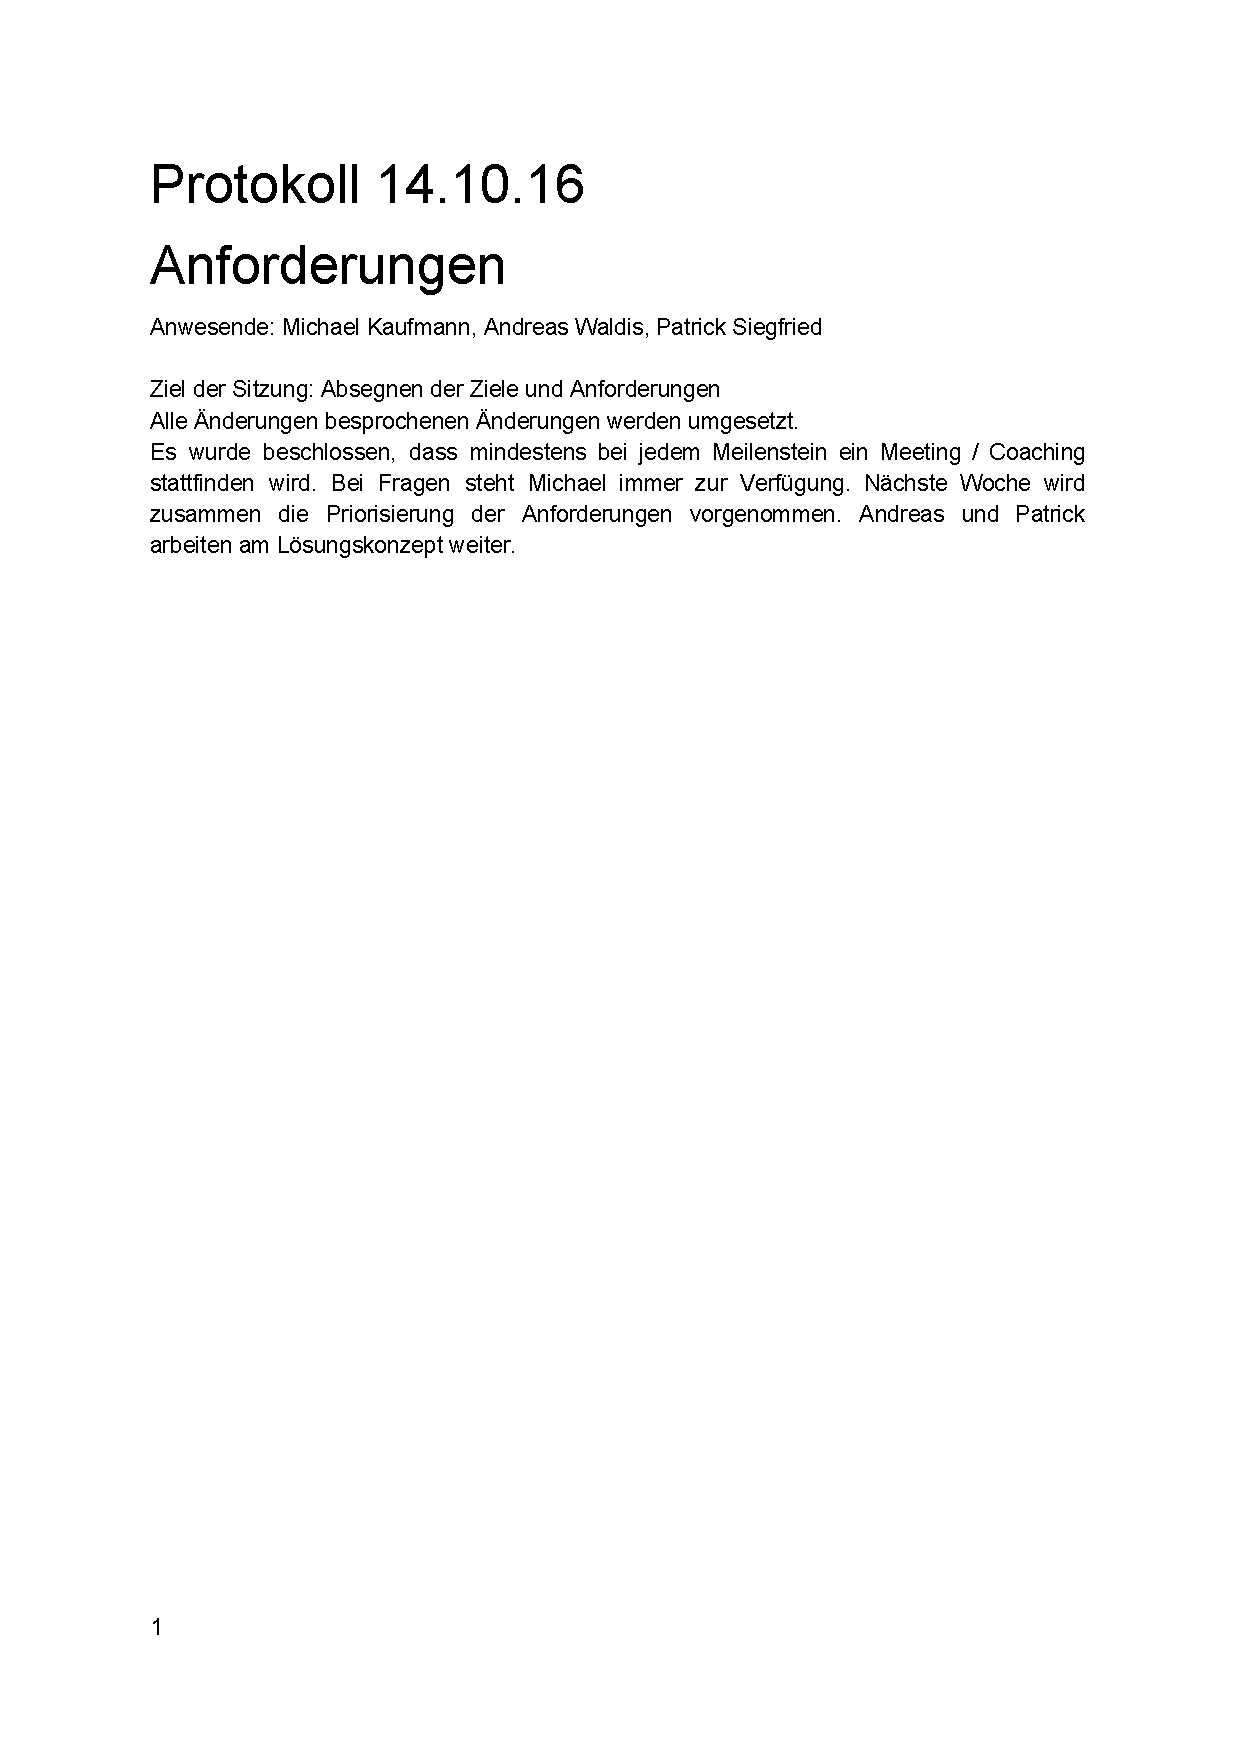
\includepdf[pages=-]{141016.pdf}

\section{Arbeitsjournal}
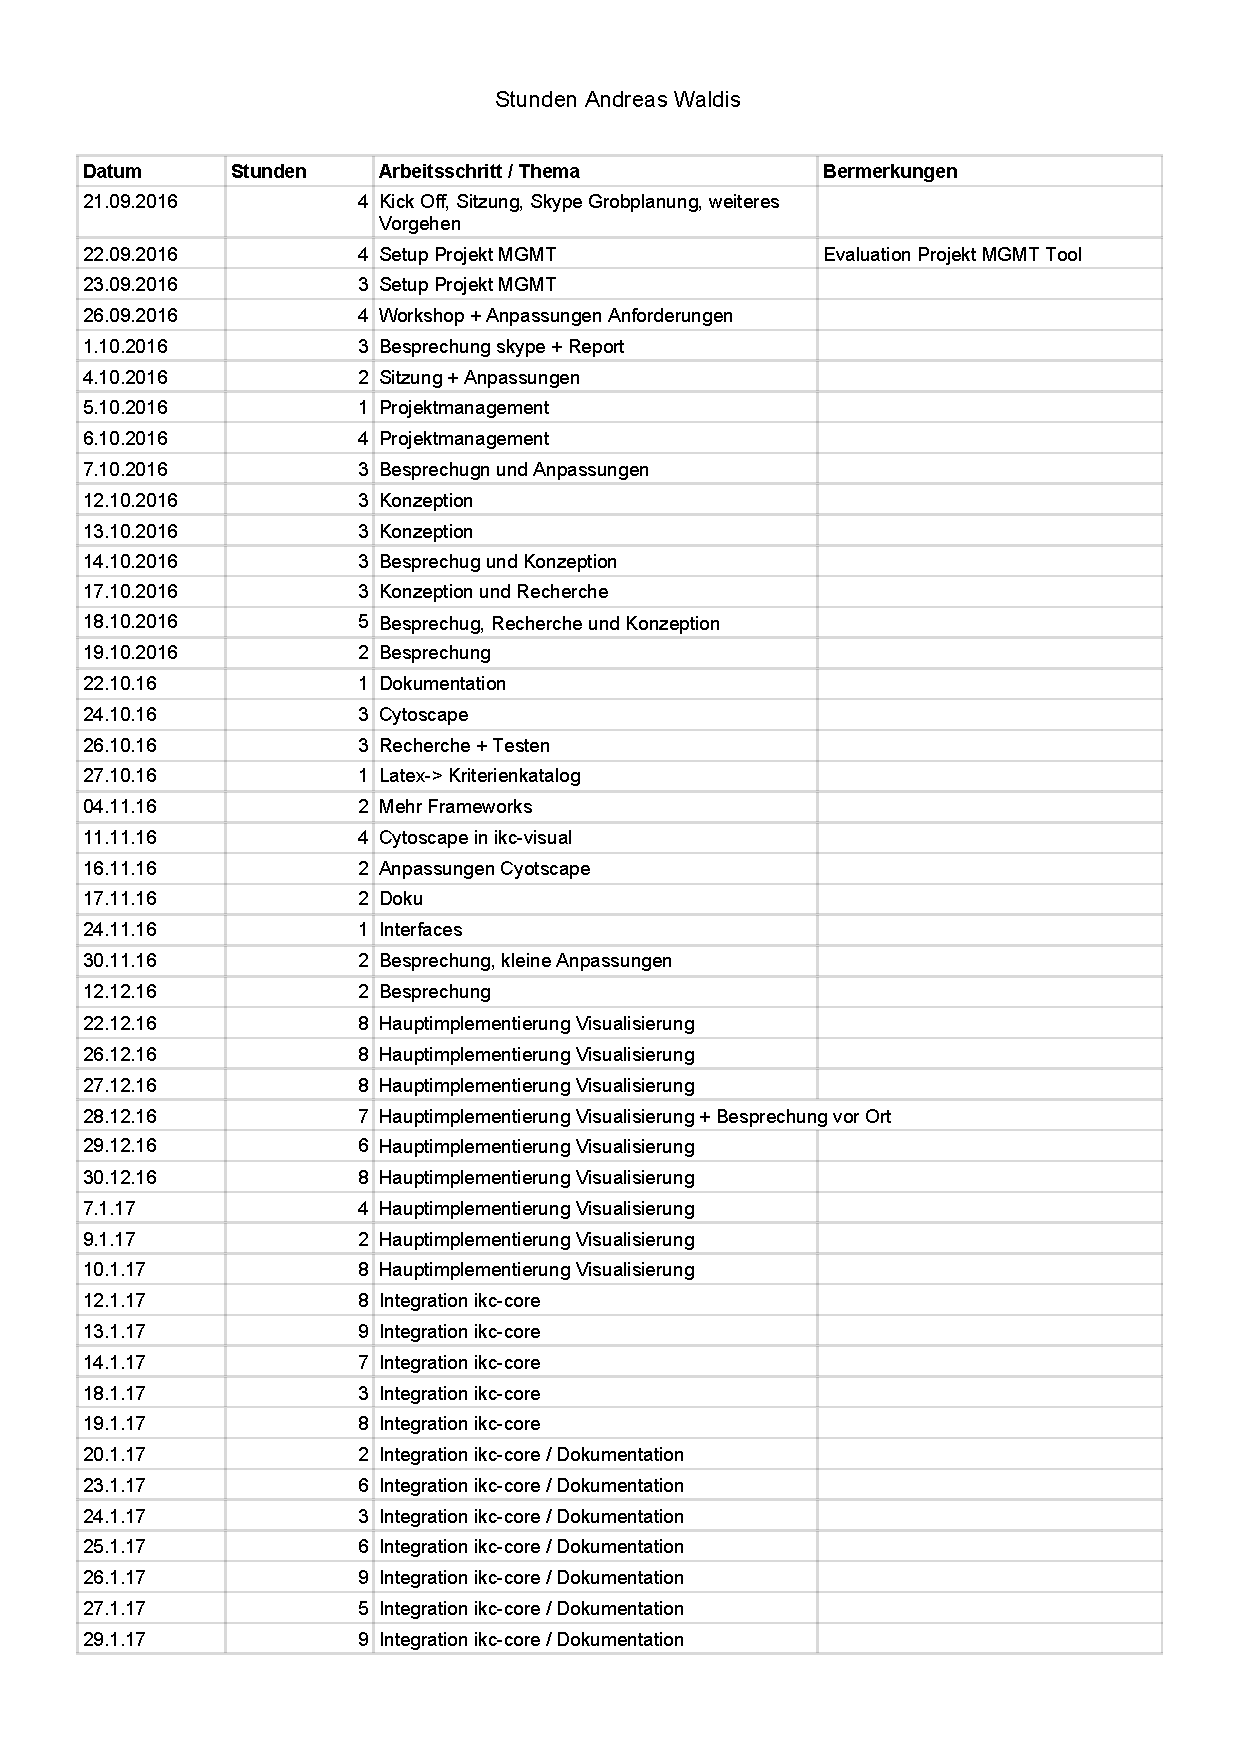
\includepdf[pages=-]{Arbeitsjournal.pdf}